\documentclass{neu_handout}
\usepackage{url}
\usepackage{amssymb}
\usepackage{amsmath}
\usepackage{marvosym}
\usepackage{graphicx}
\usepackage{subfig}
\graphicspath{ {images/} }
\everymath{\displaystyle}

% Professor/Course information
\title{Update 1}
\author{Emily Dutile, Vyshaal Narayanam, Xiwen Song, Yu Tian}
\date{November 2017}
\course{CS6220}{Data Mining Techniques}

\begin{document}

\section*{1. Problem Statement and Background}
As stated in our proposal, we look to address the following to questions:

(1) What topics are discovered frequently in reviews and do they correlate to a positive or negative review? What should a restaurant focus on to make their rating/reviews better?

(2) What neighborhoods in Pittsburgh have the best cuisine selection? Are there some areas that are more authentic, trendy or upscale than others? Based upon reviews of the top restaurants in Pittsburgh, can we recommend restaurants to a user?

\section*{2. Methods}
\subsection*{2.1 Exploratory analysis}
With the Yelp Open Dataset\footnote{\url{https://www.yelp.com/dataset}} consisting of 4.7 million reviews, 156,000 business, and 12 metropolitan areas, we needed to filter out a signification amount of data and perform some further exploration in order to set potential thresholds to either include or exclude some data.\\
To get started, we created local databases and imported the given SQL file using MySQL Server and PyCharm in our development environment. This allowed us to begin writing queries in order to better understand our dataset and possibly explore other questions. From here, we narrowed down and verified what attributes we wanted to use in order to help answer our original questions.  Using Jupyter Notebooks, we have created some basic visualizations and calculations in order to better filter, preprocess, and understand our data.\\

Below is the Yelp Dataset schema.
\begin{center}
Yelp Data Schema\\
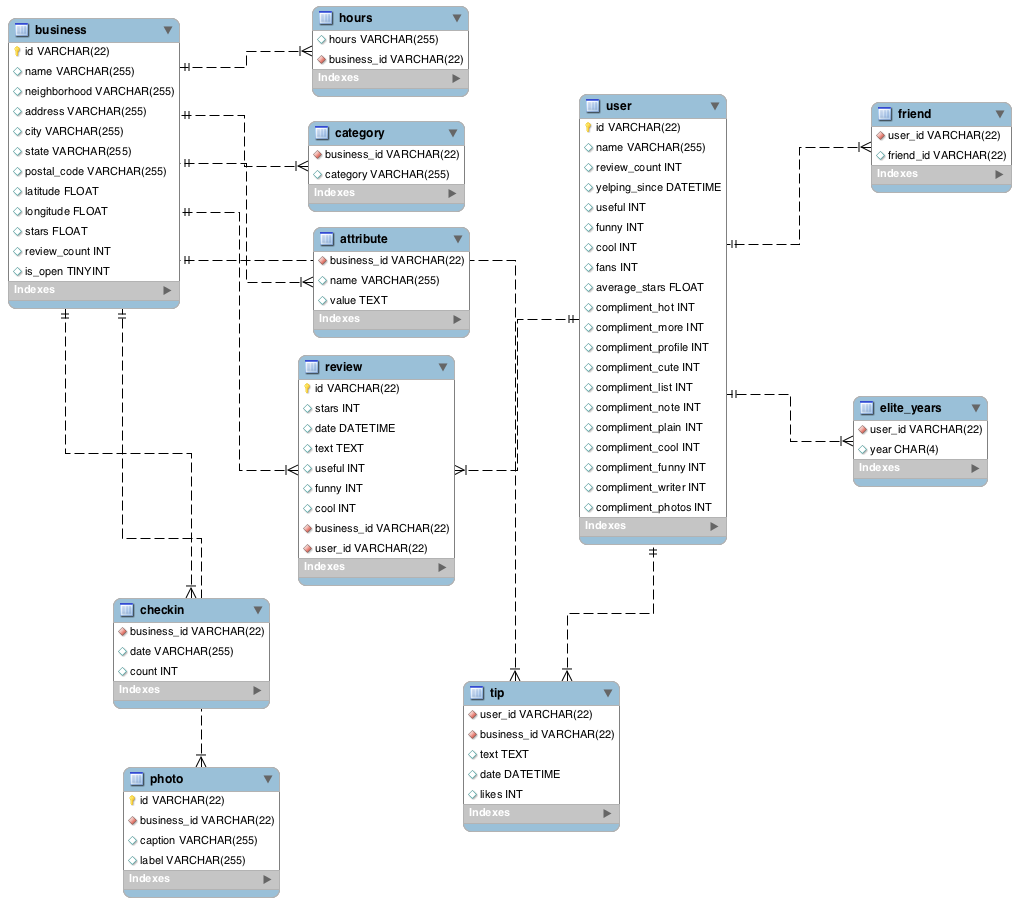
\includegraphics[width=80mm,scale=0.5]{schema}\\
\end{center}


\subsection*{2.2 Extraction}

Since Boston didn't appear to be in the data set, we first did some analysis on what other city we'd like to chose to perform the same data mining techniques on. We decided to choose Pittsburgh due to the number of restaurants (2089), the significant number of neighborhoods (53 - this includes a category of NULL for restaurants that do not have a neighborhood label), and the variety of cuisines (43 different cuisines).



\begin{center}
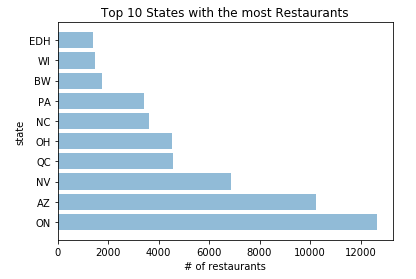
\includegraphics[width=70mm,scale=0.5]{states}
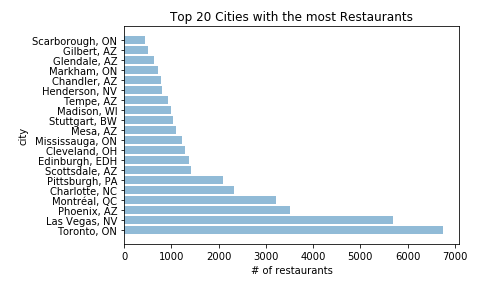
\includegraphics[width=80mm,scale=0.5]{cities}
\end{center}

\begin{center}
List of categories/cuisines: \\
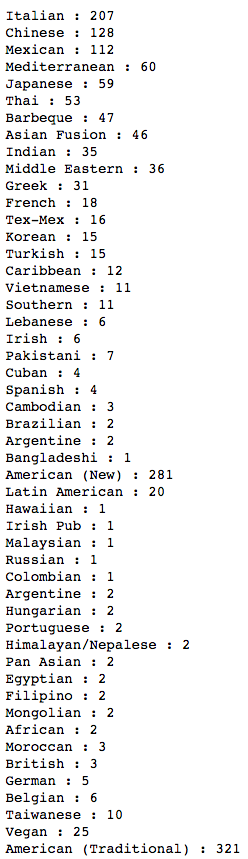
\includegraphics[width=30mm,scale=0.5]{cuisines}\\
\end{center}


In order to get a better idea of the restaurants within Pittsburgh, we created a simple visualization which plots the latitude and longitude of every restaurant.

\begin{center}
Map of Pittsburgh Restaurants \\
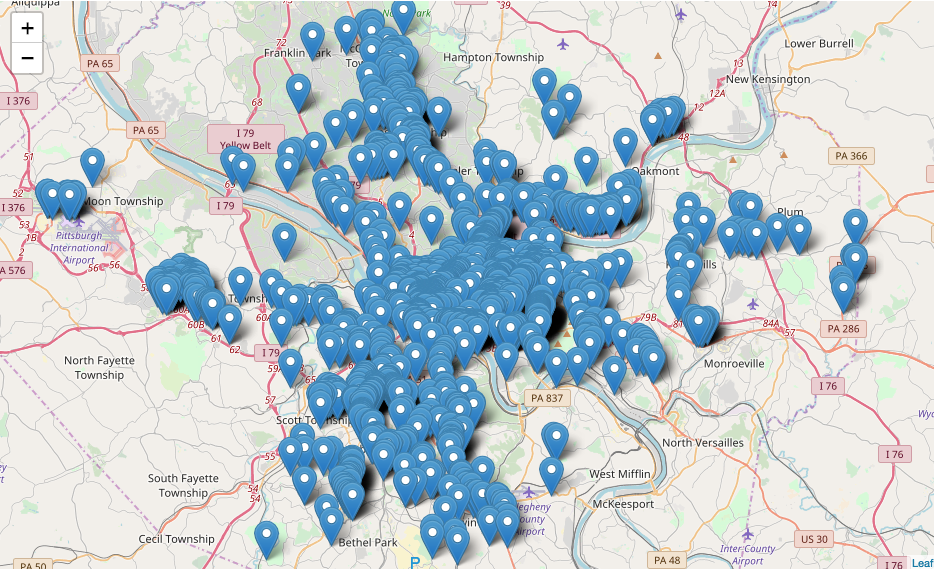
\includegraphics[width=100mm,scale=0.5]{PittsburghRestaurants}\\
\end{center}

Although interesting, this doesn't tell us too much other than it appears to be very dense around the middle of the city. Our heat map of restaurant density and the most popular restaurants in Pittsburgh do show that a lot of the neighborhoods in the center of the city are more popular.

\begin{center}
Heatmap of Restaurant Density \\
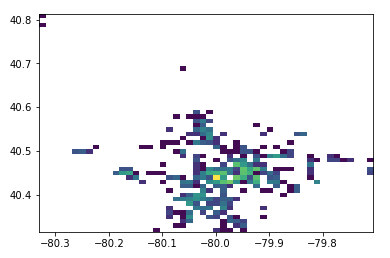
\includegraphics[width=80mm,scale=0.5]{pa_rest_density}\\
\end{center}

\begin{center}
Most popular restaurants in Pittsburgh \\
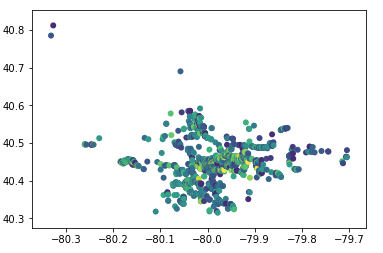
\includegraphics[width=80mm,scale=0.5]{pa_popular_restaurants}\\
\end{center}


\end{document}
